%!TEX root = main.tex
\section{Background}
This section provide technical details about the four main serverless providers, namely Amazon Web Services (\S\ref{sec:ss:aws}), Microsoft Azure (\S\ref{sec:ss:azure}), Google Cloud (\S\ref{sec:ss:google}) and IBM Cloud (\S\ref{sec:ss:ibm}). 
\vs{CHECK that this is true:} We compare the performance of all of them in our evaluation (see Section~\ref{sec:evaluation}).

%In this chapter, the choice of serverless computing providers and the choice of runtimes respectively programming languages is derived. Furthermore, the implemented tests will be explained in detail and it is shown what their effect and importance is.

%\subsection{Choosing Serverless Computing Providers}
%\label{sec:CSP}
%
%There are a lot of cloud providers available and many of them are trying to grow and therefore investing more and more in their infrastructure. So this benchmark suite could have taken into account as many cloud providers as possible, assumed they provide serverless computing, but that would have exceeded the scope of this thesis. Figure \ref{fig:market_share} illustrates on the left hand side the global revenue of the cloud infrastructure services market which has reached nearly \$23 billion in the second quarter of 2019. What's more interesting for choosing cloud providers for this benchmark suite is the market share. As one can see in figure \ref{fig:market_share} on the right hand side the market share of cloud computing is mainly dominated by a few big players: Amazon, Microsoft, Google, \gls{IBM} and Alibaba. Amazon still is the unprecedented leader in this field of business. Nevertheless, other competitors are heavily investing in the cloud business. Google will invest 3 billion euros in its European data centers as Sundar Pichai, the \gls{CEO} of Google, stated in the Google blog \cite{GoogleBlog}. And also Microsoft has recently been given a \$10 billion contract by the US Department of Defense to transform the military's cloud computing systems \cite{NYJEDI, JEDI}.
%
%\begin{figure}[htp]
%\begin{center}
%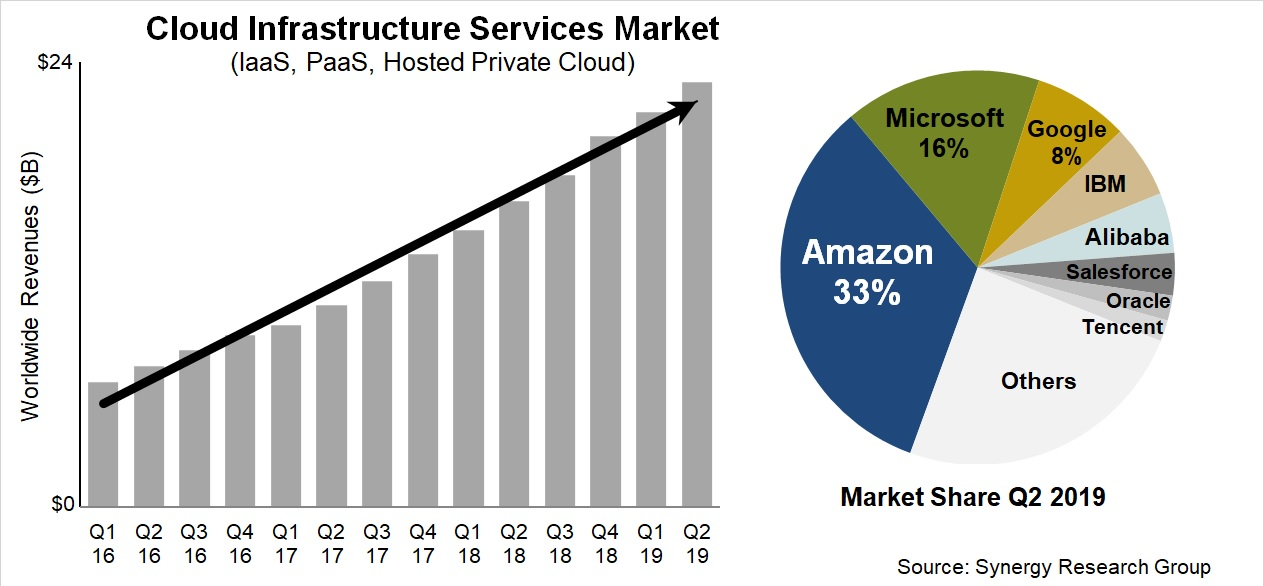
\includegraphics[width=0.5\textwidth]{bilder/synergy.jpg}
%\captionsetup[table]{justification=centering, labelfont=bf}
%\caption[Cloud Infrastructure Services Market Share]{Cloud Infrastructure Services Market Share\\Source: Synergy Research Group \cite{Synergy}}
%\label{fig:market_share}
%\end{center}
%\end{figure}
%
%For the above mentioned reasons, the following top four providers were taken into consideration.
%\begin{itemize}
%  \item Amazon Web Services
%  \item Microsoft Azure
%  \item Google Cloud
%  \item IBM Cloud
%\end{itemize}
%All of them offer a serverless platform which will be described for each cloud provider in the following sections.

%\begin{remark}
%At the beginning of this thesis, a deployment on Apache OpenWhisk was considered on the private cluster of the university of Neuchâtel. After several time wasting and failed attempts to set up OpenWhisk and contradicting documentation on the OpenWhisk website respectively the GitHub page of OpenWhisk the idea was dropped. Since \gls{IBM} uses an implementation based on OpenWhisk, the performance is expected to be similar. Nevertheless, it would have been interesting to compare those two very similar or even identical systems on a private and on a public cloud.
%\end{remark}

\subsection{Amazon Web Services Lambda}\label{sec:ss:aws}

\gls{AWS} Lambda~\cite{AWSLambda} was released in November in 2014 \cite{AWSLambdaRelease}. 
\gls{AWS} Lambda spans 18 geographically dispersed regions, plus China\cite{AWSRegions}. 
At the time of writing, it supports six different runtimes and seven different programming languages \cite{AWSLambdaLanguages}. 
Depending on the region where the function is deployed, Lambda supports up to 3000 instances to serve the user' functions~\cite{AWSLambdaScaling}. 
The memory allocated to a function instance can vary from 128 \gls{MB} up to 3008 \gls{MB} in steps of 64 \gls{MB}~\cite{AWSLambdaConfig}. 
The \gls{CPU} power increases linearly with its memory allocation.
Forinstance, at 1792 \gls{MB} the function will get 1 \gls{vCPU}~\cite{AWSLambdaConfig}.\vs{MAISSEN: why 1792?}

As observed in~\cite{216063}, Lambda executes functions using two different \gls{CPU}s, namely Intel Xeon E5-2666 clocked at 2.90 \gls{GHz}  and the Intel Xeon E5-2680, clocked at 2.80 \gls{GHz} respectively. 
%This information was extracted by Wang et al. from the file \texttt{/proc/cpuinfo} in the Linux operating system.
%\begin{remark} From my own experience I can tell that cloud providers generally don't like to tell their customers every detail of hardware they use or how exactly services are implemented. The first point might be true because they don't want to tell a customer what exact \gls{CPU}s he gets, because then he will certainly complain if it differs from the specification and the provider has to take responsibility. The second point should be obvious for economic and competition related reasons.
%\end{remark}
%Knowing that, one can more or less estimate the theoretical computing power that the virtual \gls{CPU} will provide. 
%\begin{remark}
%The pricing of \gls{AWS} Lambda and all the other services will be discussed in section \ref{sec:pricing} Pricing.
%\end{remark}

\subsection{Microsoft Azure Functions}\label{sec:ss:azure}

Microsoft Azure Functions~\cite{AzureFunctions} was released publicly in Novenber 2016~\cite{AzureFunctionsAnnouncement}. %in preview (Microsoft's term for beta) and then later in November 2016 it became generally available \cite{AzureFunctionsAnnouncement}. 
it supports five runtimes and seven different programming languages~\cite{AzureFunctionsLanguages}.
Compared to the other three cloud providers, Azure offers three different hosting plans \cite{AzureFunctionsPlans}:
%Something a little different with Azure compared to the other three cloud providers is that one can select between three different hosting plans \cite{AzureFunctionsPlans}:
Azure Functions offers billing plans that adapt to the load and popularity of the deployed function (\emph{e.g.}, the consumption plan), plans with finer-grain control over the computing instance size and pre-warming support (\emph{e.g.}, a premium plan), and an billing plan customized on a given application needs (\emph{e.g.}, the app service plan). 
This work only considers the consumption plan (generation 2.0~\cite{AzureFunctionsGenerations}), being the only one to be fully managed by the cloud provider and the most similar in the features to the ones offered by the alternative provders. 
%\begin{itemize}
%\item[] \textbf{Consumption plan:} It adds and removes instances dynamically depending on the load on the function and cost only arise when functions are running. This is the most 'serverless' option among those three.
%\item[] \textbf{Premium plan:} The premium plan is similar to the consumption plan but offers more integration and control over the functions. Instance sizes can be chosen and instances can be pre-warmed. The cost is calculated with \gls{CPU} and \gls{GB} memory used per second.
%\item[] \textbf{App Service plan:} How many and on which \gls{VM}s the functions run can be decided in the App Service plan. Scaling happens manually, time based or based on metrics such as \gls{CPU} usage.
%\end{itemize}
%This thesis will only consider the consumption plan, as it is the default plan and fully managed, and therefore \textit{more} serverless than the others. Additionally, it is similar to the services of the other providers.\\
%There are currently three different generations of the service available \cite{AzureFunctionsGenerations}, this project uses generation 2.

Azure Functions can use as many as 200 instances and up to 1.5GB memory~\cite{AzureFunctionsPlans}. 
The service can run either on Windows or Linux hosts, and is offered in 28 out of 46 publicly accessible regions~\cite{AzureRegions}.
Note that the consumption plan is only available in 11 regions for both Linux and Windows, hence we restrict to those in our experiments.
Computing nodes can be characterized by their \gls{ACU}, with 100 ACU roughly map to 1 \gls{vCPU}.
%For computing power, Azure has its own term named \gls{ACU} index, where 100 ACU roughly map to 1 \gls{vCPU}.
%The instances in the Azure functions consumption plan have an \gls{ACU} of 100 which is about the equivalent of 1 \gls{vCPU}. 
According to our investigations, we believe Azure Functions to be executed by virtual machiens of type \textit{Av2}\vs{which ones from \url{https://aws.amazon.com/ec2/instance-types/}? Clarify.}, as it most closely resembles its declared \gls{ACU}~\cite{AzureFunctionsVMs}. 
These \gls{VM}s use three different \gls{CPU}s: Intel Xeon 8171M at 2.1 \gls{GHz}, Intel Xeon E5-2673 v4 at 2.3 \gls{GHz} and Intel Xeon E5-2673 v3 at 2.4 \gls{GHz}~\cite{AzureFunctionsVMs}.

\subsection{Google Cloud Functions}\label{sec:ss:google}
%\vs{STOPPED HERE}
%On the Google Cloud Platform, the serverless service is simply called \textit{Functions} \cite{GoogleFunctions}. 
Google Functions~\cite{GoogleFunctions} was released on July in 2018~\cite{GoogleFunctionsReleases}, and currently available through seven out of twenty regions~\cite{GoogleFunctionsLocations}.
%Compared to AWS and Azure that is two and a half years respectively one year later for the first release. 
It currently only supports three programming languages~\cite{GoogleFunctionsLanguages}, namely \vs{FIX}. 
While there is not a maximum number of allocated instances per single function, it only allows up to 1000 functions to be executed concurrently~\cite{GoogleFunctionsQuotas}.
%The documentation does not mention a limit of maximum allocated instances per function. 
%However, it states that at maximum 1000 functions can be concurrently in execution \cite{GoogleFunctionsQuotas}.
Table~\ref{table:google_functions_cpu_ram} summarizes the options for CPU and memory combinations supported by the platform\cite{GoogleFunctionsPricing}.
While the official \emph{Functions} documentation lacks details on the exact CPU models, a quick inspection of \texttt{/proc/cpuinfo} unveils certain details, such as \texttt{vendor\_id}, \texttt{cpu\_family} and \texttt{model}.
We report on the use of Intel-based processors as well as some specific generation details in \vs{FIX? where?}.
%Possible options for CPU and memory allocation per instance are shown in table \ref{table:google_functions_cpu_ram} \cite{GoogleFunctionsPricing}. 
%The service is available in seven out of twenty regions~\cite{GoogleFunctionsLocations}.

\begin{table}[!t]

\caption[Google Cloud Functions - Possible memory allocation and corresponding CPU frequency]{Google Cloud Functions - Possible memory allocation and corresponding CPU frequency~\cite{GoogleFunctionsPricing}.}
%\captionsetup[table]{justification=centering, labelfont=bf}
\centering
\resizebox{\columnwidth}{!}{
\begin{tabular}{l|r|r|r|r|r} 
 \hline
	\textbf{Memory} & 128\gls{MB} & 256\gls{MB} & 512\gls{MB} & 1024\gls{MB} & 2048\gls{MB} \\ 
	\textbf{CPU} & 200\gls{MHz} & 400\gls{MHz} & 800\gls{MHz} & 1.4 \gls{GHz} & 2.4 \gls{GHz} \\
	\hline
\end{tabular}
\vspace{-10pt}
}
\label{table:google_functions_cpu_ram}
\end{table}

%Google does not mention what type of CPU they use for functions on the underlying infrastructure. 
%The CPU type could also not be extracted by Wang et al. \cite{216063} and the file \texttt{/proc/cpuinfo} does not show information on the CPU model name. 
%It shows however information for the fields \texttt{vendor\_id}, \texttt{cpu\_family} and \texttt{model}. 
%Those values reveal that Intel processors are used and can give an indication from which generation the CPU is. 
%\vs{See the example file content \ref{lst:cpuinfo} in the appendix.} 

\subsection{IBM Cloud Functions}\label{sec:ss:ibm}

\gls{IBM}'s Cloud Functions \cite{IBMFunctions} is built atop Apache OpenWhisk, an open source serverless cloud platform using Docker containers~\cite{OpenWhisk}. 
As such, in addition to Docker, it supports eight additional runtimes~\cite{IBMRuntimes}, such as \vs{FIX}.
%\gls{IBM} Cloud Functions supports nine different runtimes including a Docker runtime \cite{IBMRuntimes}. 
The service is restricted to 1000 concurrently active executions (including those enqueued for execution) per namespace~\cite{IBMLimits}. 
%However this limit can be increased for a specific business case but needs to be applied for via the ticketing system of the \gls{IBM} support \cite{IBMLimits}. 
Memory allocation can be set from 128 \gls{MB} to 2048 \gls{MB} in steps of 32 \gls{MB}. 
\gls{IBM} Cloud Functions is available in five out of six regions \cite{IBMLocations}.\footnote{One region\vs{which one?} lacks support for Cloud Foundry~\cite{IBMCloudFoundry} and as such it not be used to deply via the \gls{CLI}, and hence it is not included in this work.} 
%The documentation does not mention anything on \gls{CPU} or machines they are using. 
Our experiments revelaed that some of the  instances supporting the execution of the functions run on top of Intel Xeon E5-2683 v3 at 2.00 \gls{GHz}.
\vs{See the example file content \ref{lst:cpuinfo2} in the appendix.}

\section{Choosing Runtimes}
After the technical description and specification of each provider, the following section will deduct which runtimes respectively programming languages were chosen and why.\\
Table \ref{table:programming_languages} shows an overview of all supported runtimes for each cloud service provider mentioned in section \ref{sec:CSP}. On the right hand side there is the sum for each runtime, which indicates the number of cloud service providers supporting that runtime.

\begin{table}[htp]
\centering
\captionsetup[table]{justification=centering, labelfont=bf}
\resizebox{\columnwidth}{!}{
\begin{tabular}{|l|c|c|c|c|c||l|} 
 \hline
 & \multirow{2}{*}{AWS} & \multicolumn{2}{c|}{Azure} & \multirow{2}{*}{Google} & \multirow{2}{*}{IBM} & \multirow{2}{*}{Sum} \\ \cline{3-4}
  & & Linux & Windows & & & \\ \hline
  Node.js &  \cellcolor{green!25}yes & \cellcolor{green!25}yes & \cellcolor{green!25}yes & \cellcolor{green!25}yes & \cellcolor{green!25}yes & 4.0 \\ \hline
  Python & \cellcolor{green!25}yes & \cellcolor{green!25}yes & \cellcolor{red!25}no & \cellcolor{green!25}yes & \cellcolor{green!25}yes & 3.5 \\ \hline
  .NET Core & \cellcolor{green!25}yes & \cellcolor{green!25}yes & \cellcolor{green!25}yes & \cellcolor{red!25}no & \cellcolor{green!25}yes & 3.0 \\ \hline
  Go & \cellcolor{green!25}yes & \cellcolor{red!25}no & \cellcolor{red!25}no & \cellcolor{green!25}yes & \cellcolor{green!25}yes & 3.0 \\ \hline
  Java & \cellcolor{green!25}yes & \cellcolor{red!25}no & \cellcolor{green!25}yes & \cellcolor{red!25}no & \cellcolor{green!25}yes & 2.5 \\ \hline
  Ruby & \cellcolor{green!25}yes & \cellcolor{red!25}no & \cellcolor{red!25}no & \cellcolor{red!25}no & \cellcolor{green!25}yes & 2.0 \\ \hline
%  PowerShell & \cellcolor{green!25}yes & \cellcolor{red!25}no & \cellcolor{green!25}yes & \cellcolor{red!25}no & \cellcolor{red!25}no & 1.5 \\ \hline
  Swift & \cellcolor{red!25}no & \cellcolor{red!25}no & \cellcolor{red!25}no & \cellcolor{red!25}no & \cellcolor{green!25}yes & 1.0 \\ \hline
  PHP & \cellcolor{red!25}no & \cellcolor{red!25}no & \cellcolor{red!25}no & \cellcolor{red!25}no & \cellcolor{green!25}yes & 1.0 \\ \hline
  Docker & \cellcolor{yellow!25}ECS & \cellcolor{green!25}yes & \cellcolor{red!25}no & \cellcolor{yellow!25}Cloud Run & \cellcolor{green!25}yes & 1.5 \\
 \hline
\end{tabular}
}
\caption[Supported runtimes in serverless computing]{Supported runtimes in serverless computing.  Data source: \cite{AWSLambdaLanguages, AzureFunctionsLanguages, GoogleFunctionsLanguages, IBMRuntimes}\\ \textbf{Remark:} Since Azure has Linux and Windows as underlying \gls{OS}, only half a point is counted per \gls{OS}.}
\label{table:programming_languages}
\end{table}

It is obviously more interesting to compare runtimes and programming languages that are supported in multiple clouds and are therefore directly comparable. As the table \ref{table:programming_languages} shows Node.js is supported in each cloud, Python in all except Azure with Windows as \gls{OS}, .NET Core in all but Google and so forth. For this thesis, the top four runtimes where chosen to limit the scope. A brief summary of each runtime will be given in the following subsections.
\begin{remark}
Azure has currently 3 generations of its function service available. generation 1 is currently in maintenance mode and generation 2 and 3 are generally available. The available runtimes in the next section will only consider generation 2 (which is also used in this project):
\end{remark}

\subsection{Node.js}

Node.js is a JavaScript runtime and is built on Chrome's V8 JavaScript engine \cite{Nodejs}. As the name indicates, JavaScript is a scripting language and was first released on the 4th December 1995 by Netscape \cite{JavaScript}. It was mostly used in addition to \gls{HTML} and \gls{CSS} in web browsers \cite{JavaScript}. Because of the Node.js framework and the \gls{NPM}, JavaScript is nowadays a popular language to implement all kinds of applications. Table \ref{table:nodejs} shows supported Node.js versions of each cloud provider. 

\begin{table}[htp]
\centering
\captionsetup[table]{justification=centering, labelfont=bf}
\begin{tabular}{|l|c|c|c|c|} 
 \hline
 Node.js & AWS & Azure & Google & IBM \\ \hline
6.x  & \cellcolor{red!25}no    & \cellcolor{red!25}no    & \cellcolor{yellow!25}yes  & \cellcolor{red!25}no\\ \hline
8.x  & \cellcolor{red!25}no & \cellcolor{green!25}yes & \cellcolor{green!25}yes   & \cellcolor{green!25}yes \\ \hline
10.x & \cellcolor{green!25}yes & \cellcolor{green!25}yes & \cellcolor{yellow!25}yes  & \cellcolor{green!25}yes \\ \hline
12.x & \cellcolor{green!25}yes & \cellcolor{red!25}no & \cellcolor{red!25}no & \cellcolor{red!25}no \\ \hline
\end{tabular}
\caption[Supported Node.js runtimes]{Supported Node.js runtimes. Data source: \cite{AWSLambdaLanguages, AzureFunctionsLanguages, GoogleFunctionsLanguages, IBMRuntimes}\\ \textbf{Remark:} The yellow color means \textit{deprecated} and \textit{beta} for version 6.x respectively 10.x.}
\label{table:nodejs}
\end{table}

This benchmark suite will deploy all Node.js applications in version 10 as all providers support this version. In particular, \gls{AWS} uses version 10.x \cite{AWSLambdaLanguages}, Azure does not specify more than version 10 \cite{AzureFunctionsLanguages}, Google uses version 10.15.3 \cite{GoogleFunctionsRuntimes} and \gls{IBM} implements version 10.15.0 \cite{IBMRuntimes}.

\begin{remark}
Google has Node.js version 10 still in beta while Node.js version 8 End-of-life was on December 31, 2019 \cite{NodejsReleases}.
\end{remark}

\subsection{Python}

Python is a universal, open-source and very popular programming language. It was released in 1991 and created by Guido van Rossum \cite{PythonIntro} and runs basically anywhere \cite{PythonAbout}. Python was designed to be very easy to learn and to have readable code \cite{PythonIntro}. It only uses indentation and whitespaces to define the scope of loops, functions and classes \cite{PythonIntro}. Because of those characteristics, developers can implement new features very fast. Cuong Do, software architect of YouTube, said: "Python is fast enough for our site and allows us to produce maintainable features in record times, with a minimum of developers." \cite{PythonQuotes}. Table \ref{table:python} shows which of the four cloud provider supports which Python versions.

\begin{table}[htp]
\centering
\captionsetup[table]{justification=centering, labelfont=bf}
\begin{tabular}{|l|c|c|c|c|} 
 \hline
 Python & AWS & Azure & Google & IBM \\ \hline
2.7  & \cellcolor{green!25}yes    & \cellcolor{red!25}no    & \cellcolor{red!25}no  & \cellcolor{green!25}yes\\ \hline
3.6  & \cellcolor{green!25}yes & \cellcolor{green!25}yes & \cellcolor{red!25}no   & \cellcolor{green!25}yes \\ \hline
3.7 & \cellcolor{green!25}yes & \cellcolor{green!25}yes & \cellcolor{green!25}yes  & \cellcolor{green!25}yes \\ \hline
3.8 & \cellcolor{green!25}yes & \cellcolor{red!25}no & \cellcolor{red!25}no  & \cellcolor{red!25}no  \\ \hline
\end{tabular}
\caption[Supported Python runtimes]{Supported Python runtimes. Data source: \cite{AWSLambdaLanguages, AzureFunctionsLanguages, GoogleFunctionsLanguages, IBMRuntimes}}
\label{table:python}
\end{table}

All clouds support version 3.7, therefore this version will be used in the benchmark functions.

\subsection{Go}
Go is a procedural open source programming language developed by a team at Google and other contributors \cite{GoDoc, GoProject}. It is a relatively new language and was first released in March 2012 \cite{GoProject}. It is compiled and therefore more efficient than interpreted languages and it has good concurrency mechanisms to benefit from today's multi-core architecture \cite{GoDoc}. Go also has a garbage collector in contrast to C \cite{GoDoc}. On the Go website the following statement can be found: "It's a fast, statically typed, compiled language that feels like a dynamically typed, interpreted language." \cite{GoDoc}. Today, Go is a popular language given that is is easy to learn and write like Python but also very efficient like C. Table \ref{table:go} shows the supported Go versions.

\begin{table}[htp]
\centering
\captionsetup[table]{justification=centering, labelfont=bf}
\begin{tabular}{|l|c|c|c|c|} 
 \hline
 Go & AWS & Azure & Google & IBM \\ \hline
1.11  & \cellcolor{green!25}yes    & \cellcolor{red!25}no    & \cellcolor{green!25}yes  & \cellcolor{green!25}yes\\ \hline
\end{tabular}
\caption[Supported Go runtimes]{Supported Go runtimes. Data source: \cite{AWSLambdaLanguages, AzureFunctionsLanguages, GoogleFunctionsLanguages, IBMRuntimes}\\ \textbf{Remark:} AWS supports all versions of Go 1.x, depending on the version the binary was compiled with and deployed to Lambda.}
\label{table:go}
\end{table}

This thesis will use Go 1.11 for its benchmark functions.
\subsection{.NET Core}

.NET Core is a free and open-source software framework developed by Microsoft and its community \cite{.NETCore}. The first version was released in June 2016 \cite{.NETCoreReleases}. It supports as languages C\texttt{\#}, F\texttt{\#} and Visual Basic \cite{.NETAbout} and is currently on version 3.1 which was released in December 2019 \cite{.NETCoreBlog}. Microsoft has declared its love for Linux when Satya Nadella in the end of 2014 at a Microsoft Cloud Briefing in San Francisco presented a slide which stated "Microsoft  Linux". \cite{MicrosoftCloudBlog}. Since then the company has embraced Linux, open-source software and cross-platform support. Table \ref{table:dotnet} shows supported .NET Core versions.

\begin{table}[htp]
\centering
\captionsetup[table]{justification=centering, labelfont=bf}
\begin{tabular}{|l|c|c|c|c|} 
 \hline
 .NET Core & AWS & Azure & Google & IBM \\ \hline
2.1  & \cellcolor{green!25}yes    & \cellcolor{red!25}no    & \cellcolor{red!25}no  & \cellcolor{red!25}no\\ \hline
2.2  & \cellcolor{red!25}no    & \cellcolor{green!25}yes    & \cellcolor{red!25}no  & \cellcolor{green!25}yes\\ \hline
3.1  & \cellcolor{red!25}no    & \cellcolor{red!25}no    & \cellcolor{red!25}no  & \cellcolor{red!25}no\\ \hline
\end{tabular}
\caption[Supported .NET Core runtimes]{Supported .NET Core runtimes. Data source: \cite{AWSLambdaLanguages, AzureFunctionsLanguages, GoogleFunctionsLanguages, IBMRuntimes}}
\label{table:dotnet}
\end{table}

Because there is no common supported version, this project will use 2.1 on \gls{AWS} and 2.2 on Azure and \gls{IBM}. The language the test functions are implemented is C\texttt{\#}.

\section{Test Functions}
\label{sec:tests}
This section will briefly explain all the implemented test functions, what they test and how they are implemented. All the functions are implemented with a \gls{HTTP} trigger, since it is one that all clouds support and is the easiest to test across all platforms. For the same programming language and the same test, the implementation will vary from cloud to cloud a little bit. This is due to slightly different function calls and return statements each cloud defines on their own. However, these differences are not relevant regarding performance results.
\subsection{Latency Test}
\label{subsec:latency}
The latency test  is fairly simple. The function is called and then immediately returns a small \gls{JSON} body with \gls{HTTP} status code 200. The test function is intended to be as fast and simple as possible to measure latency for each cloud and runtime. The following code listing \ref{code:latency} shows exemplary the implementation of the latency test on \gls{AWS} in Node.js.

\begin{minipage}{\linewidth}
\lstset{escapeinside={<@}{@>}}
\begin{lstlisting}[frame=single,caption={Latency test implementation on AWS in Node.js},label=code:latency,linewidth=.82\textwidth,xleftmargin=.18\textwidth]
  exports.handler <@\textcolor{javascriptbrown}{=}@> <@\textcolor{javascriptpurple}{function}@>(<@\textcolor{javascriptblue}{event}@>, <@\textcolor{javascriptblue}{context}@>, <@\textcolor{javascriptblue}{callback}@>) {
      <@\textcolor{javascriptpurple}{const}@> <@\textcolor{javascriptblue}{res}@> <@\textcolor{javascriptbrown}{=}@> {
          statusCode: <@\textcolor{javascriptroyalblue}{200}@>,
          headers: {
              <@\textcolor{javascriptred}{'Content-Type'}@>: <@\textcolor{javascriptred}{'application/json'}@>
          },
          body: JSON.stringify({
              success: <@\textcolor{javascriptpurple}{true}@>,
              payload: {
                  <@\textcolor{javascriptred}{'test'}@>: <@\textcolor{javascriptred}{'latency test'}@>,
              }
          })
      };
    <@\textcolor{javascriptblue}{callback}@>(<@\textcolor{javascriptpurple}{null}@>, <@\textcolor{javascriptblue}{res}@>);
  }
\end{lstlisting}
\end{minipage}

\subsection{CPU Test (Factorization)}
\label{sec:factors_test}
This test describes the first of the two \gls{CPU} tests. The \gls{CPU} is the component of a system which does effectively do the calculations of a program. It is therefore the most important criterion of serverless computing and logically also the most expensive. This test is targeting mostly the \gls{CPU} by calculating all integer factors/divisors imperatively of an integer number. Listing \ref{code:factors} shows pseudo code of such a number factorization.

\begin{minipage}{\linewidth}
\lstset{escapeinside={<@}{@>}}
\begin{lstlisting}[frame=single,caption={Factorization test pseudo code},label=code:factors,linewidth=.75\textwidth,xleftmargin=.25\textwidth]
  for(i = 1; i < SquareRoot(Number), i++) {
      if(Number modulo i == 0) {
          factors.add(i)
          if(Number / i != i) {
              factors.add(Number / i)
          }
      }
  }
\end{lstlisting}
\end{minipage}

The algorithm works as follows: one iterates from 1 to the square root of the number $N$ to be factorized. For each value $i$ it is tested if $N$ is dividable by $i$ without rest (modulo operator). If so, a factor of $N$ has been found and $i$ is added to the results. In addition, if $N$ divided by $i$ does not equal $i$ itself, the matching part $x$ of $i$ has also been found where $x \cdot i = N$. This is also the reason why only the numbers up to the square root of $N$ need to be considered. The algorithm has a complexity of $\mathcal{O}(n^{\frac{1}{2}})$.

\begin{remark}
The algorithm is not to be confused with prime factorization. In this case, all factors of a number are calculated but with prime factorization only prime numbers are calculated. The approach and results share some characteristics.
\end{remark}

\subsection{CPU Test (Matrix Multiplication)}
The matrix multiplication is the second \gls{CPU} test in this benchmark suite. The user can input a number $n$ which defines the width and height of two matrices. The two matrices are both filled with random integer numbers between 0 and 100. The product of those two matrices is calculated by multiplication. The algorithm is defined in listing \ref{code:matrix} in pseudo code.

\begin{minipage}{\linewidth}
\lstset{escapeinside={<@}{@>}}
\begin{lstlisting}[frame=single,caption={Matrix multiplication test pseudo code},label=code:matrix,linewidth=0.8\textwidth,xleftmargin=.2\textwidth]
  matrixA = randomMatrix[n][n]
  matrixB = randomMatrix[n][n]
  matrixMult = [n][n];
  
  for(i = 0; i < matrixA.height; i++) {
      for(j = 0; j < matrixB.width; j++) {
          sum = 0;
          for(k = 0; k < matrixA.width; k++) {
              sum += matrixA[i][k] * matrixB[k][j];
          }
          matrixMult[i][j] = sum;
      }
  }
\end{lstlisting}
\end{minipage}
\newline

First, two matrices of height and width $n$ are defined and filled with random integer numbers from 0 to 100. Also an empty matrix for the result is initialized. For each field of the resulting matrix one needs to calculate the dot product of row $i$ from matrix $A$ and column $j$ of matrix $B$. This is achieved by multiplying each field of row $i$ from matrix $A$ with each field of column $j$ from matrix $B$ and accumulating the sum over $k$. The sum is then stored as field $i,j$ in the resulting matrix. The algorithm has a complexity of $\mathcal{O}(n^{3})$.
\subsection{I/O Test}
The fourth test in this benchmark suite is a disk test. Each serverless cloud provides a temporary file system which the functions can use. The function can for example write a file with some intermediate results which it will later read again for further use. Other function calls which run in the same instance share this file system and can also access the file. Given that serverless tends to be or should be stateless, the feature of a temporary storage is not of great importance. Nevertheless, specific applications might benefit from such a feature and therefore it is included in this thesis. I/O operations are often expensive and in a synchronous function that can lead to \gls{CPU} wait.\\
The implementation of the test is fairly simple. Listing \ref{code:filesystem} shows the pseudo code of the test.


\begin{minipage}{\linewidth}
\lstset{escapeinside={<@}{@>}}
\begin{lstlisting}[frame=single,caption={I/O test pseudo code},label=code:filesystem,linewidth=0.75\textwidth,xleftmargin=.25\textwidth]
  text = ""
    
  for(i = 0; i < s; i++) {
      text += "A";
  }
  
  startWrite = Time.Now()
  for(i = 0; i < n; i++) {
      writeFile(i+'.txt', text, 'utf-8');
  }
  endWrite = Time.Now()
  
  startRead = Time.Now()
  for(i = 0; i < n; i++) {
      file = readFile(i+'.txt', 'utf-8');
  }
  endRead = Time.Now()
  
  writeTime = endWrite - startWrite
  readTime = endRead - startRead
\end{lstlisting}
\end{minipage}
\newline

The algorithm writes files and then reads them. It takes two input parameters $n$ defining the number of files and $s$ the size of each file in bytes. A string \texttt{text} is generated with length equal to $s$. Since the encoding used is \texttt{utf-8} each normal character takes 8 bits or 1 byte of storage. Then $n$ many files are written to the file system. After that all the written files are read. Both these operations are timed and the result will be the time it took to write respectively read the files. The complexity of the algorithm is $\mathcal{O}(n)$.

\subsection{Custom Test}
Last but not least there is a customizable test. The objective of this test is that the user can easily implement his own function and then benchmark it. The skeleton is provided for each one of the four clouds in each of the four languages. A timer is included to measure the execution time which can later be further analysed.